\documentclass[]{article}
\usepackage{lmodern}
\usepackage{amssymb,amsmath}
\usepackage{ifxetex,ifluatex}
\usepackage{fixltx2e} % provides \textsubscript
\ifnum 0\ifxetex 1\fi\ifluatex 1\fi=0 % if pdftex
  \usepackage[T1]{fontenc}
  \usepackage[utf8]{inputenc}
\else % if luatex or xelatex
  \ifxetex
    \usepackage{mathspec}
  \else
    \usepackage{fontspec}
  \fi
  \defaultfontfeatures{Ligatures=TeX,Scale=MatchLowercase}
\fi
% use upquote if available, for straight quotes in verbatim environments
\IfFileExists{upquote.sty}{\usepackage{upquote}}{}
% use microtype if available
\IfFileExists{microtype.sty}{%
\usepackage{microtype}
\UseMicrotypeSet[protrusion]{basicmath} % disable protrusion for tt fonts
}{}
\usepackage[a4paper,top=2.5cm,bottom=2.5cm,left=3.5cm,right=2.5cm]{geometry}
\usepackage{hyperref}
\PassOptionsToPackage{usenames,dvipsnames}{color} % color is loaded by hyperref
\hypersetup{unicode=true,
            pdftitle={ECOWAS Common Currency, a Mirage or Possibility?},
            pdfauthor={Sagiru Mati1, Irfan Civcir2*, Hüseyin Özdeşer3},
            colorlinks=true,
            linkcolor=blue,
            citecolor=green,
            urlcolor=blue,
            breaklinks=true}
\urlstyle{same}  % don't use monospace font for urls
\usepackage{longtable,booktabs}
\usepackage{graphicx,grffile}
\makeatletter
\def\maxwidth{\ifdim\Gin@nat@width>\linewidth\linewidth\else\Gin@nat@width\fi}
\def\maxheight{\ifdim\Gin@nat@height>\textheight\textheight\else\Gin@nat@height\fi}
\makeatother
% Scale images if necessary, so that they will not overflow the page
% margins by default, and it is still possible to overwrite the defaults
% using explicit options in \includegraphics[width, height, ...]{}
\setkeys{Gin}{width=\maxwidth,height=\maxheight,keepaspectratio}
\IfFileExists{parskip.sty}{%
\usepackage{parskip}
}{% else
\setlength{\parindent}{0pt}
\setlength{\parskip}{6pt plus 2pt minus 1pt}
}
\setlength{\emergencystretch}{3em}  % prevent overfull lines
\providecommand{\tightlist}{%
  \setlength{\itemsep}{0pt}\setlength{\parskip}{0pt}}
\setcounter{secnumdepth}{5}
% Redefines (sub)paragraphs to behave more like sections
\ifx\paragraph\undefined\else
\let\oldparagraph\paragraph
\renewcommand{\paragraph}[1]{\oldparagraph{#1}\mbox{}}
\fi
\ifx\subparagraph\undefined\else
\let\oldsubparagraph\subparagraph
\renewcommand{\subparagraph}[1]{\oldsubparagraph{#1}\mbox{}}
\fi

%%% Use protect on footnotes to avoid problems with footnotes in titles
\let\rmarkdownfootnote\footnote%
\def\footnote{\protect\rmarkdownfootnote}

%%% Change title format to be more compact
\usepackage{titling}

% Create subtitle command for use in maketitle
\providecommand{\subtitle}[1]{
  \posttitle{
    \begin{center}\large#1\end{center}
    }
}

\setlength{\droptitle}{-2em}

  \title{ECOWAS Common Currency, a Mirage or Possibility?}
    \pretitle{\vspace{\droptitle}\centering\huge}
  \posttitle{\par}
    \author{Sagiru Mati\textsuperscript{1}, Irfan Civcir\textsuperscript{2}*, Hüseyin Özdeşer\textsuperscript{3}}
    \preauthor{\centering\large\emph}
  \postauthor{\par}
    \date{}
    \predate{}\postdate{}
  
\usepackage[hang,flushmargin]{footmisc}
%\usepackage{footmisx}
%\usepackage{footnotebackref}
\usepackage{acronym}
\usepackage{secdot}
\usepackage{hyperref}
\usepackage{footnotehyper}    % It allows hyperref, unlike footmisc package
%\usepackage{UTF-8}{inputenc}
\usepackage{parskip}
%\usepackage[a4paper,top=2in,bottom=2in,left=3in,right=2in]{geometry}
\usepackage{longtable}
\usepackage{booktabs}
\usepackage{xcolor}
\usepackage{natbib}
\usepackage[font=bf,labelfont=bf]{caption} %to edit captions
\usepackage[section]{placeins}
\usepackage{setspace}
\usepackage{chngcntr}
\usepackage{float}
\usepackage{fontspec}
\setmainfont{Arial}
%\usepackage{helvet}
\usepackage{float}
\setlength{\floatsep}{3pt plus 2pt minus 2pt}
\setlength{\textfloatsep}{3pt plus 2pt minus 2pt}
\setlength{\intextsep}{3pt plus 2pt minus 2pt}
%\renewcommand{\familydefault}{\sfdefault}
\doublespacing
%\counterwithin{figure}{section}
%\counterwithin{table}{section}
%\counterwithin{equation}{section}
\parskip6pt
%\usepackage[nolists]{endfloat} %to put all floats at the end of a document
%\renewcommand{\efloatseparator}{\mbox{}} % change the spacing of endfloat
\usepackage{flafter} %to put all floats after their first reference in a document
\usepackage{booktabs}
\usepackage{longtable}
\usepackage{array}
\usepackage{multirow}
\usepackage{wrapfig}
\usepackage{float}
\usepackage{colortbl}
\usepackage{pdflscape}
\usepackage{tabu}
\usepackage{threeparttable}
\usepackage{threeparttablex}
\usepackage[normalem]{ulem}
\usepackage{makecell}
\usepackage{xcolor}

\begin{document}
\maketitle

\thispagestyle{empty}

\textsuperscript{1}Faculty of Economics and Administrative Sciences, Near East University, North Cyprus, \href{mailto:sagirumati@gmail.com}{\nolinkurl{sagirumati@gmail.com}}

\textsuperscript{2}Faculty of Polical Science, Ankara University, Turkey, \href{mailto:civcir@politics.ankara.edu.tr}{\nolinkurl{civcir@politics.ankara.edu.tr}}.

\textsuperscript{3}Faculty of Economics and Administrative Sciences, Near East University, North Cyprus, \href{mailto:huseyinozdeser@neu.edu.tr}{\nolinkurl{huseyinozdeser@neu.edu.tr}}

\begin{center} 

\section*{ABSTRACT}

\end{center}

\newacro{ECOWAS}{Economic Community of West African States} \ac{ECOWAS} members have been working towards creating a monetary union since 1975. \ac{ECOWAS} members adopted a resolution in 2007, which introduced ECOWAS Vision 2020. This study attempts to provide the economic reasons why this vision is a mirage or possibility. Unlike the previous studies, the interaction of global, regional and domestic inflation rates is used to assess the feasibility of actualizing \ac{ECOWAS} Vision 2020 aimed at creating a monetary union. With the help of \newacro{SVAR}{Structural Vector Autoregression} \ac{SVAR} using \newacro{BQ}{Blanchard and Quah} \ac{BQ}decomposition over the sample of 1975:05 to 2018:08, questions pertaining to symmetry of inflationary shocks, dominance of regional shocks and response of domestic inflation to a given shock are assessed. Impulse response, variance decomposition as well as correlation of domestic inflationary shocks are employed to assess whether this vision is a mirage or possibility. It is found that although the vision is a mirage, creating a common currency can serve as a shock absorber against the negative spillovers of global and regional inflationary shocks. The study recommends that Nigeria can be part of the WAEMU and that more coordination among ECOWAS members is needed before actualizing this vision.

\textbf{Keywords:} Monetary Union, Optimal Currency Area, ECOWAS, WAEMU, SVAR, \ac{BQ} Decomposition.

\textbf{JEL classification:} C13, E31, E52, E58, F33, F42.

\vskip60pt

\hrulefill

*Corresponding Author: \href{mailto:civcir@politics.ankara.edu.tr}{\nolinkurl{civcir@politics.ankara.edu.tr}}
\clearpage
\pagestyle{plain}
\pagenumbering{arabic}

\hypertarget{introduction}{%
\section{Introduction}\label{introduction}}

After establishment of the \newacro{EMU}{European Monetary Union} \ac{EMU} which led to the creation of Euro as single currency, several groups of countries attempt to follow suit. One of these groups of countries is Economic Community of West African States (ECOWAS, or it's French and Portuguese abbreviation CEDEAO)\footnote{ECOWAS official languages are English, French and Portuguese.} , which is similar to the European Union (EU) in terms of structure and operation. After the Treaty of Lagos signed on 28th May, 1975, members of ECOWAS have been working towards creating a common central bank, single currency similar to Euro to be called Eco, and unified monetary policy. In order to accomplish this objective, ECOWAS in June 2007 adopted a resolution, which introduced ECOWAS Vision 2020. Some economic criteria known as convergence criteria, similar to Maastricht Treaty of the EMU, are adopted in the name of \emph{Decision A/DEC.17/12/01} in December, 2001. These criteria were modified in \emph{Supplementary Act A/SA/4/06/12} of 29\textsuperscript{th} June, 2012 on convergence agreement and macroeconomic stability between ECOWAS Member States (ECOWAS, \protect\hyperlink{ref-ECOWAS2017}{2017}). The Convergence criteria contain two categories, primary criteria and secondary criteria. The primary criteria stipulate that deficit-GDP ratio should be less than 3 per cent, annual average inflation rate less than 10 per cent, gross external reserves greater than 3 months of imports. The secondary criteria require that debt-GDP ratio to be lower than 70 per cent, Central bank financing of the budget deficit should not be above 10 per cent of the previous year's tax revenue, and variation of nominal exchange rate to be within the band of ±10 per cent. This study attempts to provide the economic reasons why this vision is a mirage or possibility. Towards this end, this study is grounded on the \newacro{OCA}{Optimum Currency Areas} \ac{OCA}, the theory developed by Mundell (\protect\hyperlink{ref-mundell1961theory}{1961}), McKinnon (\protect\hyperlink{ref-McKinnon1963}{1963}) and Kenen (\protect\hyperlink{ref-kenen1969theory}{1969}) to explain the economic conditions necessary for a beneficial monetary unification.
OCA is one of the theories used to assess the costs and benefits of forming or joining \newacro{MU}{monetary union} an MU (Bayoumi \& Eichengreen, \protect\hyperlink{ref-BAYOUMI1997761}{1997}; Capie \& Wood, \protect\hyperlink{ref-capie2003monetary}{2003}; Plasmans, Engwerda, Van Aarle, Di Bartolomeo, \& Michalak, \protect\hyperlink{ref-plasmans2006dynamic}{2006}), or the nature of macroeconomic shocks among the members of an MU (see for example, De Grauwe, \protect\hyperlink{ref-de2000monetary}{2000}; Chow \& Kim, \protect\hyperlink{ref-Chow2003}{2003}; Khamfula \& Huizinga, \protect\hyperlink{ref-khamfula2004southern}{2004}; Lee \& Azali, \protect\hyperlink{ref-lee2012east}{2012}; Legrand, \protect\hyperlink{ref-LEGRAND2014136}{2014}; Regmi, Nikolsko-Rzhevskyy, \& Thornton, \protect\hyperlink{ref-Regmi2015}{2015}; Zhao \& Kim, \protect\hyperlink{ref-Zhao2009}{2009}). Some of the conditions proposed by \ac{OCA} for a beneficial monetary unification include symmetry of shocks and similar business cycle among the members of the \ac{MU}. The higher the compatibility of an MU with \ac{OCA}, the larger the benefit to all members, and vice versa (De Grauwe, \protect\hyperlink{ref-de2000monetary}{2000}). The magnitude of benefit or cost of joining an MU depends on the frequency, nature, and transmission of the shocks which impact the \ac{MU}. If the nature of the shocks is symmetric (asymmetric), the benefit (cost) of joining \ac{MU} is substantial (Plasmans et al., \protect\hyperlink{ref-plasmans2006dynamic}{2006}).

Despite this giant vision, there exist very few empirical studies to examine the possibility or otherwise of actualizing this vision. Moreover, these studies employ other methodologies than the \ac{BQ} decomposition and focus on \newacro{CFZ}{CFA Franc Zone} \ac{CFZ}\footnote{Monetary union of Francophone countries whose economies are linked to the French franc.} and \newacro{WAMZ}{West African Monetary Zone} \ac{WAMZ}, see for example (Fielding \& Shields, \protect\hyperlink{ref-Fielding2005}{2005}; Hefeker, \protect\hyperlink{ref-hefeker2010fiscal}{2010}; Masson \& Pattillo, \protect\hyperlink{ref-masson2001monetary}{2001}; Tsangarides \& Qureshi, \protect\hyperlink{ref-TSANGARIDES20081261}{2008}). It differs from other similar studies in terms of methodology, variables, data frequency and sample size. This paper attempts to empirically establish whether the \ac{ECOWAS}'s vision 2020 is a mirage or possibility in the light of OCA. For this the study attempts to answer the following research questions; i. Do members of the ECOWAS meet the primary and secondary convergence criteria?; ii. Are the shocks in ECOWAS countries symmetric?; iii. Is the members' source of shocks regional?; iv. Are the responses of ECOWAS countries to a given shock similar? If the answer to each of the above set of questions is no (yes), then the implication is that ECOWAS's Vision 2020 is a mirage (possibility). Having either yes or no as an answer to the individual question implies different conclusion from having either yes or no to all the questions. Having yes (no) as an answer to the second and fourth questions, individually or collectively, implies that the ECOWAS members are ready (not ready) for a single monetary policy. On the other hand, having yes (no) as an answer to question 3 signifies that the ECOWAS members could benefit (suffer) from using a single currency.

\hypertarget{overview-of-ecowas}{%
\section{Overview of ECOWAS}\label{overview-of-ecowas}}

The organization currently comprises fifteen (15) member countries. They include Benin (BEN), Burkina Faso (BFA), Cote d'Ivoire (CIV), Guinea Bissau (GNB), Mali (MLI), Niger (NER), Senegal (SEN), Togo (TGO), the Gambia (GMB), Ghana (GHA), Guinea (GUI), Nigeria (NGA), Sierra Leone (SLE), Cabo Verde (CPV) and Liberia (LBR), see Masson and Pattillo (2001). The West African Economic and Monetary Union (WAEMU) is made up of the first eight members, while the last two are not part of any monetary union. The remaining members comprise the West African Monetary Zone (WAMZ)\footnote{WAEMU and WAMZ were established in 1994 and 2000 respectively.}. Only three Member States, namely Guinea, Liberia and Nigeria met the first of the primary criteria (deficit-GDP ratio less than 3 per cent) as opposed to six in 2015, which were Benin (6.2\%), the Gambia (9.5\%), Ghana (10.9\%) Niger (6.1\%), Sierra Leone (6.4\%) and Togo (8.5\%). As for the second of the primary criteria (annual average inflation less than 10 per cent), only Ghana, Nigeria, and Sierra Leone recorded an inflation rate of more than ten percent (10\%) in 2016. In 2015, all ECOWAS members other than Ghana recorded an inflation rate of less than 10\%. The Anglophone countries recorded higher inflation rates. The higher inflation rates could be attributable to the depreciation of the currencies of these members in 2015 and 2016. The target of the third primary criterion (gross external reserves greater than 3 months of imports) was previously six months of imports, but was reduced to three months of import in 2015. In 2016, only the Gambia (2.4 months), Ghana (2,8 months) and Guinea (1.4 months) did not meet this criterion. Nigeria (6.5 months) and Cabo Verde (6.4 months) had the largest coverage of imports in both 2015 and 2016 (ECOWAS, \protect\hyperlink{ref-ECOWAS2017}{2017}).

Only Cabo Verde (128.6\%), The Gambia (117.3\%) and Togo (79.4\%) have not met the first of the secondary criteria (debt-GDP ratio lower than 70 per cent). Guinea, Nigeria, the Gambia and Sierra Leone did not meet the second of the secondary criteria (Central bank financing of deficit above 10 per cent of the previous year's tax revenue). Regarding the third secondary criterion (variation of nominal exchange rate within the band of ±10 per cent), three currencies in 2016, compared to two in 2015, experienced an average variation outside the ±10\% band. The affected currencies are Guinea franc (16.4\%), Nigerian naira (23.5\%) and Sierra Leone leone (19.1\%) as reported by (ECOWAS, \protect\hyperlink{ref-ECOWAS2017}{2017}).

\hypertarget{literature-review}{%
\section{Literature review}\label{literature-review}}

The preconditions of forming an MU guided by the OCA include the existence of symmetry of shocks across all the members (Mundell, \protect\hyperlink{ref-mundell1961theory}{1961}), open economies (Kenen, \protect\hyperlink{ref-kenen1969theory}{1969}) as well as well-diversified economies (McKinnon, \protect\hyperlink{ref-McKinnon1963}{1963}). Hsu (\protect\hyperlink{ref-hsu2010common}{2010}) and Regmi et al. (\protect\hyperlink{ref-Regmi2015}{2015}) highlight the common empirical methodologies for operationalizing the OCA: Agbeyegbe (\protect\hyperlink{ref-agbeyegbe2008feasibility}{2008}), for example, assesses the \emph{convergence criteria} of the MU candidates, Chow \& Kim (\protect\hyperlink{ref-Chow2003}{2003}) assesses the nature of (a)symmetry of macroeconomic shocks, analyzing the correlation of macroeconomic variables of the potential MU members (see for example, Rana, \protect\hyperlink{ref-RANA2007711}{2007}).

Employing fractional integration and cointegration as econometric methodology, Alagidede, Coleman, \& Cuestas (\protect\hyperlink{ref-ALAGIDEDE2012460}{2012}) find the existence of significant heterogeneity in the behavior of inflation among the WAMZ countries. They suggested the enhancement of policy coordination among central banks the members before signing the treaty for a single currency. In contrast to other studies, Debrun, Masson, \& Pattillo (\protect\hyperlink{ref-debrun2005monetary}{2005}) develop and calibrate a model in which the incentives to join an MU is provided by the negative spillover from the independent monetary policy. They identified lack of fiscal convergence as the main hindrance of actualizing an MU in West Africa. Their findings are in contradiction with the conclusions of other studies, which identify that asymmetric shocks or low level of regional trade as the main constraints of establishing the MU. Correlation analysis was employed by Fielding, Lee, \& Shields (\protect\hyperlink{ref-Fielding2004}{2004}) to establish that monetary integration among the members of \ac{CFZ}led to the improvement of macroeconomic integration. After applying both soft and hard clustering algorithms on some variables, selected based on OCA and convergence criteria, Tsangarides \& Qureshi (\protect\hyperlink{ref-TSANGARIDES20081261}{2008}) examine the suitability of an MU among WAMZ as well as ECOWAS countries. The outcome of their cluster analysis shows significant dissimilarities among the MU candidates, especially the WAMZ countries. They further reveal that it would be costly for Ghana and Nigeria to be in WAMZ because they are `singletons'. Hefeker (\protect\hyperlink{ref-hefeker2010fiscal}{2010}) examines how fiscal policy, structural reform, and monetary union interact. His conclusions reveal that symmetric monetary policy may play a role in influencing fiscal authorities to adopt a distortionary fiscal policy, which subsequently reduces their structural reform effort. He further argues that asymmetric monetary union causes further polarization among the member countries. Gros \& Thygesen (\protect\hyperlink{ref-gros1998european}{1998}) and Chown (\protect\hyperlink{ref-chown2003history}{2003}) provide the historical account of monetary arrangement in the world, (Kunroo, \protect\hyperlink{ref-Kunroo2015}{2015}) explores the most recent literature survey on OCA.

In the light of the foregoing literature review, it could be safe to argue that no study employs OCA in conjunction with BQ decomposition to analyze the mirage (possibility) of forming an MU among the ECOWAS members. The studies that utilize this methodology mostly focus on the Asian countries (see, Chow \& Kim, \protect\hyperlink{ref-Chow2003}{2003}; Hsu, \protect\hyperlink{ref-hsu2010common}{2010}; Lee \& Azali, \protect\hyperlink{ref-lee2012east}{2012}) and the European countries (see Eichengreen \& Bayoumi, \protect\hyperlink{ref-eichengreen1996asia}{1996}; Boivin, Giannoni, \& Mojon, \protect\hyperlink{ref-Boivin2008}{2008}; Legrand, \protect\hyperlink{ref-LEGRAND2014136}{2014}). It is believed that employing BQ decomposition can provide further insight into the mirage or possibility of the ECOWAS members to form a full-fledged MU.

\hypertarget{data-and-methodology}{%
\section{Data and Methodology}\label{data-and-methodology}}

The monthly series of \newacro{CPI}{Consumer Price Index} \ac{CPI}\footnote{The base year is 2010} which is used to calculate the inflation rate is obtained from International Financial Statistics (IFS). Annual percentage change in CPI measures the inflation level\footnote{\(π_t^i=(lnX_t-lnX_{t-12}) \times 100\)} . The CPI monthly series from May 1975 to August, 2018 is employed for the analysis. The choice of sample period reflects the date Treaty of Lagos was signed.

\newacro{GI}{Global Inflation}\ac{GI} and \newacro{RI}{Regional Inflation} \ac{RI} are calculated from the weighted averages of Global CPI and Regional CPI respectively\footnote{\(w_{i}=\frac{\overline{X}_t}{\sum_{1}^{n}\overline{X}_t} \text{, } r_t=\sum_1^nw_{it}X_{it}\text{, } g_t=\sum_1^nw_{it}X_{it}\), where \(w_i\), \(r_t\) and \(g_t\) stand for the individual weight, regional CPI, and global CPI respectively. \(X_t\) is the CPI and \(\overline{X}_t\) is the mean of the CPI, and n is the number of countries considered in the calculation of regional or global CPI}. The United States of America (USA), United Kingdom (UK), France and China are taken as global economies, because these economies exert influence on the ECOWAS countries. Some studies consider the USA to represent the global economy (see for example Chow \& Kim, \protect\hyperlink{ref-Chow2003}{2003}; Regmi et al., \protect\hyperlink{ref-Regmi2015}{2015}). Due to a lack of CPI data for some ECOWAS countries over the full sample, only eight ECOWAS countries are considered in this study. These countries include Nigeria (NGA), Gambia (GMB), Ghana (GHA), Cote d'Ivoire (CIV), Burkina Faso (BFA), Niger (NER), Senegal (SEN) and Togo (TGO). The values of CPI for Togo are missing over the range of 1995:1 and 1995:07. However, we use the forecast values from an ARIMA(2,1,2) model to create the missing values as it is important to include Togo as part of the analysis because it is one of the founders of ECOWAS. The first three countries are members of the WAMZ, and the rest are member of the WAEMU.
For the data analysis and estimation, this study uses long-run restrictions to identify the structural global shocks (GS), regional shocks (RS) and domestic shocks (DS). This form of identification is based on Blanchard \& Quah (\protect\hyperlink{ref-Blanchard1989}{1989}) decomposition which is also adopted by Chow \& Kim (\protect\hyperlink{ref-Chow2003}{2003}), Hsu (\protect\hyperlink{ref-hsu2010common}{2010}) and Regmi et al. (\protect\hyperlink{ref-Regmi2015}{2015}) . Specifically, the model involves estimating the following equation;
\small
\begin{equation}
\begin{bmatrix} 1 & \xi_{12} & \xi_{13}\\ 
\xi_{21} & 1 & \xi_{23}\\
\xi_{31} & \xi_{32} & \xi_{33}
\end{bmatrix}
\begin{bmatrix} \pi^{g}\\
\pi^{r}\\
\pi^{d}
\end{bmatrix}=\begin{bmatrix}\lambda_{11}(L) & \lambda_{12}(L) & \lambda_{13}(L)\\
\lambda_{21}(L) & \lambda_{22}(L) & \lambda_{23}(L)\\
\lambda_{31}(L) & \lambda_{32}(L) & \lambda_{33}(L) 
\end{bmatrix}
\begin{bmatrix}\pi_{t-1}^{g}\\ \pi_{t-1}^{r}\\ \pi_{t-1}^{g}
\end{bmatrix}+
\begin{bmatrix}\gamma_{11} & 0 & 0\\
0 & \gamma_{22} & 0\\
0 & 0 & \gamma_{33}
\end{bmatrix}
\begin{bmatrix}d_{1t}\\ d_{2t}\\ d_{3t}
\end{bmatrix} +
\begin{bmatrix} \varepsilon_{1t}\\ \varepsilon_{2t}\\ \varepsilon_{3t}
\end{bmatrix}
\label{eq:VAR}
\end{equation}

\large

Equation \eqref{eq:VAR} can be represented compactly as

\begin{equation}
\Xi X_{t}=\Lambda(L)X_{t-1}+\Gamma D_{t} +\varepsilon_{t} \label{eq:stable-VAR}
\end{equation}

Where \(\Xi\) represents the matrix of coefficients of the endogenous variables, \(\Lambda\) is the matrix of coefficients of the lagged endogenous variables, and \(\Gamma\) is the matrix of coefficients of the dummy variables.

Or, in reduced form:

\begin{equation}
X_{t}=\Psi X_{t-1}+\varphi D_{t}+e_{t} \label{eq:reduced-VAR}
\end{equation}

Where \(\Psi=\Xi^{-1} \Lambda (L)\), \(\varphi=\Xi^{-1} \Lambda \Gamma\) and \(e_t=\Xi^{-1} \varepsilon_{t}\).

Equation \eqref{eq:stable-VAR} is a stationary VAR with vector \(X_t\) containing the variables, specifically, global inflation (GI) \(π^g\), regional inflation (RI) \(π^r\), and domestic inflation (DI) \(π^d\). The set of dummy variables is represented by \(D_t\), which captures the break dates for GI, RI and DI. The Greek letters \(\Xi\) and \(\Lambda\) are \(\mathbb{R}^{n×n}\) matrices of parameters. Similarly, \(\varepsilon_t\) is a vector containing the inflationary shocks, GS, RS and DS. Equation \eqref{eq:stable-VAR} provides the compact representation of equation \eqref{eq:VAR} and equation \eqref{eq:reduced-VAR} is the reduced form VAR.

Using Wold representation, the vector moving average of equation \eqref{eq:VAR} can be represented as follows (Enders, \protect\hyperlink{ref-enders2015applied}{2015}).

\begin{equation}
\pi^{g}=\sum_{q=0}^{\infty}\lambda_{11}(q) \varepsilon^{g}_{t-q}+\sum_{q=0}^{\infty}\lambda_{12}(q) \varepsilon^{r}_{t-q}+\sum_{q=0}^{\infty}\lambda_{13}(q) \varepsilon^{d}_{t-q} \label{eq:G-SVAR}
\end{equation}
\begin{equation}
\pi^{r}=\sum_{q=0}^{\infty}\lambda_{11}(q) \varepsilon^{g}_{t-q}+\sum_{q=0}^{\infty}\lambda_{12}(q) \varepsilon^{r}_{t-q}+\sum_{q=0}^{\infty}\lambda_{13}(q) \varepsilon^{d}_{t-q} \label{eq:R-SVAR}
\end{equation}
\begin{equation}
\pi^{d}=\sum_{q=0}^{\infty}\lambda_{11}(q) \varepsilon^{g}_{t-q}+\sum_{q=0}^{\infty}\lambda_{12}(q) \varepsilon^{r}_{t-q}+\sum_{q=0}^{\infty}\lambda_{13}(q) \varepsilon^{d}_{t-q} \label{eq:D-SVAR}
\end{equation}

Or compactly as

\begin{equation}
\begin{bmatrix}
\pi^{g}\\
\pi^{r}\\
\pi^{d}
\end{bmatrix}=
\begin{bmatrix}
\Omega_{11} & \Omega_{12} & \Omega_{13}\\
\Omega_{21} & \Omega_{22} & \Omega_{23}\\
\Omega_{31} & \Omega_{32} & \Omega_{33} 
\end{bmatrix} \times 
\begin{bmatrix}
\varepsilon^{g}_t\\
\varepsilon^{r}_t\\
\varepsilon^{d}_t
\end{bmatrix} 
\label{eq:BMA}
\end{equation}

Where \(\Omega_{ij}=\Lambda_{ij}(L)\) is a lag operator polynomial; therefore, equation \eqref{eq:BMA} can be represented compactly as

\begin{equation}
X_{t}=\Omega (L) \varepsilon_t
\label{eq:compact-BMA}
\end{equation}

For equations \eqref{eq:BMA} and \eqref{eq:compact-BMA} to be valid, the endogenous variables have to be stationary and that the structural shocks have unit variance and are uncorrelated (Enders, \protect\hyperlink{ref-enders2015applied}{2015}; Juselius, \protect\hyperlink{ref-juselius2006cointegrated}{2006}; Lütkepohl, Krätzig, \& Phillips, \protect\hyperlink{ref-lutkepohl2004applied}{2004}). The restrictions needed for identifying this system of the equations involve the following small country assumptions\footnote{These assumptions are the same as in Chow \& Kim (\protect\hyperlink{ref-Chow2003}{2003}), Hsu (\protect\hyperlink{ref-hsu2010common}{2010}), and Regmi et al. (\protect\hyperlink{ref-Regmi2015}{2015})}; i. domestic economies are small open economies and domestic inflation has no contemporaneous and lagged effects on global inflation ii. Idiosyncratic shocks of domestic economies have zero long-run effect on both regional and global economies iii. Regional shocks have no long-run impact on the global economy. Given these small country assumptions, Equation \eqref{eq:VAR} is restricted such that \(\lambda_{13} (L)=0\), so that domestic inflation does not have both contemporaneous and lagged effects on the global inflation. Three restrictions\footnote{For just-identified VAR system, number of restrictions (r) is given by r=(n\^{}2-n)/2, where n is the number of variables in the system. Given 3 variables, the required number of restriction is 3. } need to be imposed in order to identify equation \eqref{eq:VAR}, hence the long-run restriction such that \(\Omega_{12}=\Omega_{13}=\Omega_{23}=0\) in equation \eqref{eq:BMA} is required to recover the shocks.

\hypertarget{empirical-results}{%
\section{Empirical Results}\label{empirical-results}}

For the full sample of 1975:05 to 2018:08, all the inflation variables (GI, RI and DI) appear to be I(0) except the global inflation, Nigerian inflation and Gambian inflation, based on formal unit root tests developed by Phillips \& Perron (\protect\hyperlink{ref-10.2307ux2f2336182}{1988}) and Dickey \& Fuller (\protect\hyperlink{ref-Dickey1979}{1979}). However, when structural breaks are taken into account, these integrated inflation variables become stationary. The structural breaks occurs at various dates, so a dummy variable is generated to capture each break date for each inflation variable, 1 is assigned for the specific break date and 0 otherwise\footnote{The SB dates for the global inflation is 1981:11, and 1987:01 and 1996:07 for the Gambia and Nigeria respectively}. Formally \(D_{it}=1\) for \(t=i\) and \(D_{it}=0\) for \(t\neq i\), where \(i\) is the break date. For the sake of comparison, four subsamples are considered; two samples capturing the period before and after establishment of WAEMU and other two samples covering the period before and after creation of WAMZ. New definition of global CPI, which includes China, is also used for the samples after creation of WAEMU and WAMZ because China becomes a major global player in recent years. VAR with two lags is estimated for all the countries in the form of equation \eqref{eq:reduced-VAR}\footnote{The lag selection is guided by the number of lags necessary to make the VAR stable and whiten its error.} . All the VAR models meet the diagnostic requirements of homoscedasticity, non-autocorrelation and stability\footnote{The diagnostic results are not reported in order to save space.}. The models used in this study are defined in Table \ref{tab:tab-def}\footnote{To save space, only comparison of models 2 and 3 and that of models 5 and 6 are reported. We also determine that inclusion of China as part of the global variable does make any significant difference.}

\begin{table}[t]

\caption{\label{tab:tab-def}Sample, Model and Definition of Global Variable}
\centering
\resizebox{\linewidth}{!}{
\begin{tabular}{lll}
\toprule
\multicolumn{1}{c}{\textbf{Model name}} & \multicolumn{1}{c}{\textbf{Sample}} & \multicolumn{1}{c}{\textbf{Definition of global CPI}} \\
\cmidrule(l{3pt}r{3pt}){1-1} \cmidrule(l{3pt}r{3pt}){2-2} \cmidrule(l{3pt}r{3pt}){3-3}
M1 & 1975 to 2018a & Weighted averages of CPI's of US, UK, and France used as a global CPI\\
M2 & 1975 to 1993b & Definition of global CPI same as M1\\
M3 & 1994 to 2018c & Definition of global CPI same as M1\\
M4 & 1994 to 2018c & Weighted averages of CPI's of  US, UK, France and China used as a global CPI\\
M5 & 1975 to 1999d & Definition of global CPI same as M1\\
M6 & 2000 to 2018e & Definition of global CPI same as M1\\
M7 & 2000 to 2018e & Definition global CPI same as M4\\
\bottomrule
\multicolumn{3}{l}{Note: a, b, c, d, and e stand for full sample, period before WAEMU, period after WAEMU,  period before WAMZ and period after WAMZ respectively.}\\
\end{tabular}}
\end{table}

\FloatBarrier

\hypertarget{the-impulse-response-of-domestic-inflation}{%
\subsection{The Impulse Response of Domestic Inflation}\label{the-impulse-response-of-domestic-inflation}}

The purpose of this section is to observe how domestic inflation responds to both RS and GS similar to Regmi et al. (\protect\hyperlink{ref-Regmi2015}{2015}). If the members of a monetary union respond to a given shock in a similar way, then common monetary policy could be used to address the consequence of the shocks, otherwise, each member country has to use its own monetary policy to address the shock. In essence, if the members' responses to a given shock are similar, then monetary unification is beneficial, otherwise, it is costly.

In order to gain insight into the responses of domestic economies to the regional and global shocks, impulse responses of M2 are compared with those of M3. Figure \ref{fig:FigM2M3} reports the impulse responses of M2 and M3, while Figure \ref{fig:FigM5M6} contains the impulse responses of M5 and M6. The top part of these figures represents the responses of domestic economies to global shocks, while the responses of domestic economies to regional shocks are depicted at the bottom of these figures. For simplicity of reference, M2-G implies sub-figure of M2 model showing response of domestic economies to global shocks, and M3-R signifies sub-figure of M3 model showing response of domestic economies to regional shocks.

The first task is to compare the impulse responses of models before the establishment of WAEMU (M2) and WAMZ (M5) with the corresponding models representing period after their establishment. To this end, M2 is compared with M3, while M5 is compared with M6. Before the establishment of WAEMU, M2-G shows the response of Burkina Faso to global shocks could be as high as 1.72 and the response of Niger to global shock could be as low as -1.38. On the other hand, M3-G shows that the highest response to global shocks after creation of WAEMU is 0.78 recorded by Guinea Bissau and the lowest is -0.06 recorded by Niger, indicating a fall in the magnitude of the responses by 55 per cent and 96 per cent respectively. In addition to this, M2-G and M3-G indicate that the shocks disappear at shorter horizon in the latter model than in the former. As indicated by M2-R and M3-R, the level of responses to regional shocks are lower after WAEMU creation but shocks die out faster before the establishment of the WAEMU. Moreover, the paths of the responses to global shocks are similar except for Burkina Faso, Niger and Gambia for both M2 and M3, and the paths of responses to regional shocks are also similar except for Ghana in M2 and except for Ghana, Nigeria and the Gambia in M3.

\begin{figure}[ht!]
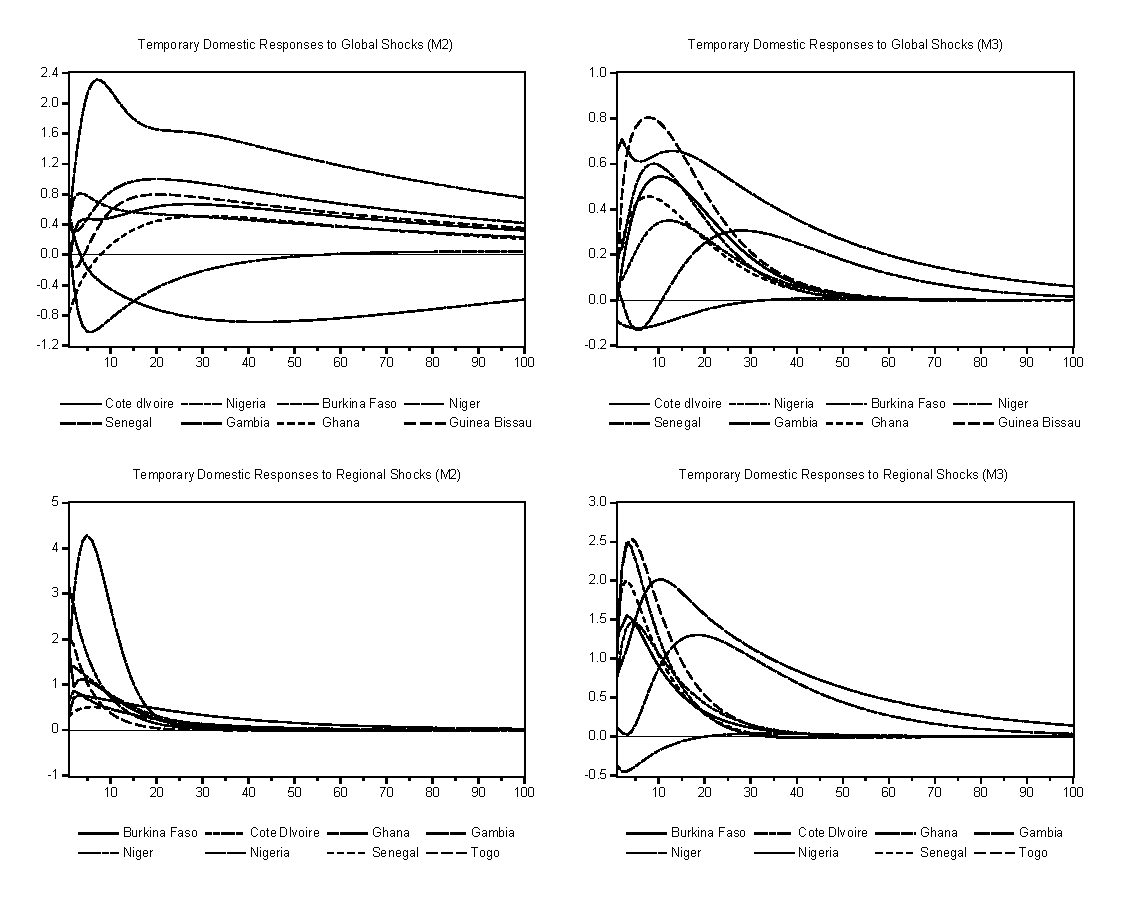
\includegraphics[width=0.98\linewidth,height=0.9\textheight]{FIGURES/figure1} \caption{Response of Domestic Economies to Regional and Global Shocks (M2 and M3)}\label{fig:FigM2M3}
\end{figure}

Figure \ref{fig:FigM5M6} attempts to compare M5 and M6 in order to find out the dynamics of the responses before and after the establishment of the WAMZ. Based on the impulse responses, period after the creation of the WAMZ has not only shown lower responses of domestic economies to both the global and regional shocks but also faster disappearance of both the shocks. Additionally, the paths of the responses to global shocks are similar except for Burkina Faso, Niger and the Gambia for both M5 and M6, and the paths of responses to regional shocks are also similar except for Nigeria and the Gambia in M5.

\begin{figure}[ht]

{\centering 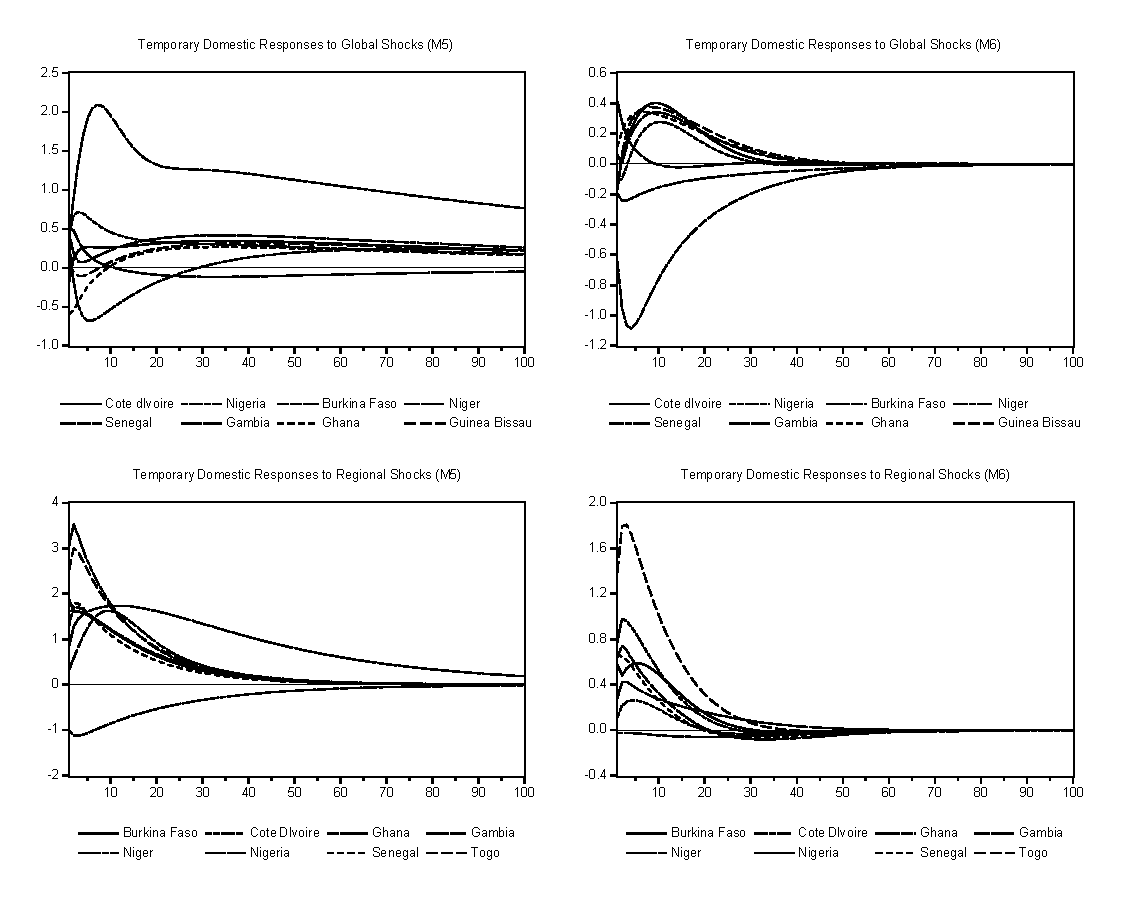
\includegraphics[width=0.98\linewidth,height=0.9\textheight]{FIGURES/figure2} 

}

\caption{Response of Domestic Economies to Regional and Global Shocks (M5 and M6)}\label{fig:FigM5M6}
\end{figure}

\FloatBarrier

\hypertarget{variance-decomposition}{%
\subsection{Variance Decomposition}\label{variance-decomposition}}

The idea is that a country should join an MU if the regional shocks dominate, opt for autonomous monetary policy if the shocks are idiosyncratic, or peg its currency against the global currency if the forecast error variance is dominated by the global shocks (Chow \& Kim, \protect\hyperlink{ref-Chow2003}{2003}; Regmi et al., \protect\hyperlink{ref-Regmi2015}{2015})

Tables \ref{tab:decomp-m2-m3} and \ref{tab:decomp-m5-m6} report the 2-month-ahead and 24-month-ahead variance forecast error of the inflation models. Comparison of M2 and M3 is presented in Table \ref{tab:decomp-m2-m3}, M5 and M6 in Table \ref{tab:decomp-m5-m6}. Again for easy reference, M2-2H denotes 2-month horizon variance decomposition of model M2, while M3-24H represents 24-month horizon variance decomposition of model M3 and so on.

Comparison of M2 and M3 in Table \ref{tab:decomp-m2-m3} provides a greater insight. The M2-2H of the table shows that only Cote D'Ivoire, Niger and Togo had some significant magnitudes of RS before the birth of WAEMU. Their RS magnitudes were 31.07, 67.05 and 50.78 (2-month horizon) and 44.77, 55.92 and 40.47 (24-month horizon) respectively. However, the scenario changed after the birth of WAEMU as only the non-WAEMU Anglophone countries are not RS-dominated. The RS for Ghana, the Gambia and Nigeria after WAEMU creation are 0.24, 13.86 and 26.26 (2-month horizon) and 26.36, 9.68 and 81.59 (24-month horizon) respectively. The implication is that most members became suitable for the common currency after the creation of the common currency.

\begin{table}[!h]

\caption{\label{tab:decomp-m2-m3}Variance decomposition of inflation, M2 and M3}
\centering
\fontsize{9}{11}\selectfont
\begin{tabu} to \linewidth {>{\raggedright}X>{\raggedright}X>{\raggedright}X>{\raggedright}X>{\raggedright}X>{\raggedright}X>{\raggedright}X>{\raggedright}X>{\raggedright}X>{\raggedright}X>{\raggedright}X>{\raggedright}X>{\raggedright}X}
\toprule
\multicolumn{1}{c}{\textbf{ }} & \multicolumn{3}{c}{\textbf{2-month horizon (M2)}} & \multicolumn{3}{c}{\textbf{2-month horizon (M3)}} & \multicolumn{3}{c}{\textbf{24-month horizon (M2)}} & \multicolumn{3}{c}{\textbf{24-month horizon (M3)}} \\
\cmidrule(l{3pt}r{3pt}){2-4} \cmidrule(l{3pt}r{3pt}){5-7} \cmidrule(l{3pt}r{3pt}){8-10} \cmidrule(l{3pt}r{3pt}){11-13}
\textbf{Country} & \textbf{GS} & \textbf{RS} & \textbf{DS} & \textbf{GS} & \textbf{RS} & \textbf{DS} & \textbf{GS} & \textbf{RS} & \textbf{DS} & \textbf{GS} & \textbf{RS} & \textbf{DS}\\
\hline
BFA & 1.93 & 13.4 & 84.67 & 1.39 & 75.56 & 23.04 & 11.97 & 23.67 & 64.36 & 17.96 & 73.51 & 8.54\\
CIV & 1.43 & 31.07 & 67.5 & 1.39 & 66.47 & 32.14 & 13.71 & 44.77 & 41.52 & 8.49 & 77.89 & 13.62\\
GHA & 2.86 & 16.39 & 80.75 & 1.24 & 0.24 & 98.52 & 6.17 & 24.45 & 69.38 & 2.93 & 26.36 & 70.7\\
GMB & 4.85 & 7.89 & 87.26 & 0.04 & 13.86 & 86.1 & 21.62 & 4.79 & 73.59 & 0.25 & 9.68 & 90.07\\
NER & 0.05 & 67.05 & 32.9 & 1.24 & 76.24 & 22.52 & 18.38 & 55.92 & 25.71 & 10.19 & 83.76 & 6.04\\
NGA & 2.07 & 2.14 & 95.8 & 1.53 & 26.26 & 72.22 & 13.15 & 3.32 & 83.53 & 0.97 & 81.59 & 17.44\\
SEN & 0.25 & 4.07 & 95.68 & 0.39 & 85.99 & 13.62 & 10.68 & 12.38 & 76.94 & 6.3 & 81.84 & 11.87\\
TGO & 0.85 & 50.78 & 48.37 & 0.87 & 32.97 & 66.16 & 19.92 & 40.47 & 39.6 & 9.29 & 59.92 & 30.79\\
\bottomrule
\end{tabu}
\end{table}

To make comparison between the period before and after the birth of WAMZ, Table \ref{tab:decomp-m5-m6} reports the variance decomposition of M5 and M6. According to M6-2H and M6-24H, Ghana, the Gambia and Nigeria are still not RS-dominated even after the creation of WAMZ, as their RS magnitudes are 45.70, 0.49 and 1.71 (2-month horizon) and 26.94, 0.30 and 5.78 (24-month horizon). This means that Anglophone countries are not ready for the common currency.

\begin{table}[!h]

\caption{\label{tab:decomp-m5-m6}\bfseries{Variance decomposition of inflation, M5 and M6}}
\centering
\fontsize{9}{11}\selectfont
\begin{tabu} to \linewidth {>{\raggedright}X>{\raggedright}X>{\raggedright}X>{\raggedright}X>{\raggedright}X>{\raggedright}X>{\raggedright}X>{\raggedright}X>{\raggedright}X>{\raggedright}X>{\raggedright}X>{\raggedright}X>{\raggedright}X}
\toprule
\multicolumn{1}{c}{ } & \multicolumn{3}{c}{**2-month horizon (M5)**} & \multicolumn{3}{c}{2-month horizon (M6)} & \multicolumn{3}{c}{24-month horizon (M5)} & \multicolumn{3}{c}{24-month horizon (M6)} \\
\cmidrule(l{3pt}r{3pt}){2-4} \cmidrule(l{3pt}r{3pt}){5-7} \cmidrule(l{3pt}r{3pt}){8-10} \cmidrule(l{3pt}r{3pt}){11-13}
\textbf{Country} & \textbf{GS} & \textbf{RS} & \textbf{DS} & \textbf{GS} & \textbf{RS} & \textbf{DS} & \textbf{GS} & \textbf{RS} & \textbf{DS} & \textbf{GS} & \textbf{RS} & \textbf{DS}\\
\hline
BFA & 1.42 & 22.41 & 76.17 & 0.83 & 22.49 & 76.68 & 3.83 & 47.36 & 48.81 & 19.22 & 44.07 & 36.71\\
CIV & 1.23 & 42.08 & 56.69 & 0.68 & 9.77 & 89.55 & 4.97 & 69.18 & 25.85 & 23.66 & 19.83 & 56.51\\
GHA & 1.52 & 0.69 & 97.79 & 4.47 & 45.7 & 49.83 & 5.08 & 7.63 & 87.29 & 4.2 & 26.94 & 68.86\\
GMB & 2.39 & 20.48 & 77.13 & 0.44 & 0.49 & 99.08 & 12.35 & 18.16 & 69.49 & 0.12 & 0.3 & 99.58\\
NER & 0.04 & 78.35 & 21.61 & 0.62 & 37.29 & 62.09 & 0.97 & 88.28 & 10.75 & 10.79 & 53.01 & 36.2\\
NGA & 1.59 & 11.5 & 86.91 & 0.62 & 1.71 & 97.67 & 6.18 & 27.62 & 66.2 & 0.68 & 5.78 & 93.54\\
SEN & 0.18 & 39.81 & 60.01 & 1.3 & 39.38 & 59.32 & 1.21 & 55.78 & 43.01 & 16.44 & 33.12 & 50.44\\
TGO & 0.38 & 66.18 & 33.44 & 2.11 & 27.51 & 70.38 & 0.69 & 81.11 & 18.2 & 3.6 & 49.27 & 47.13\\
\bottomrule
\end{tabu}
\end{table}

\FloatBarrier

\hypertarget{correlation-of-domestic-shocks}{%
\subsection{Correlation of domestic shocks}\label{correlation-of-domestic-shocks}}

This section employs correlation to determine the symmetry or otherwise of the inflationary shocks. The residuals from the SVAR for each country are taken to be the shocks; DS, RS and GS. If the correlation is zero, negative or small, then the shocks are asymmetric, but if they are strongly positive, then they are said to be symmetric (Hsu, \protect\hyperlink{ref-hsu2010common}{2010}). The correlation estimates of RS and GS are not reported as it is observed that they are all strongly positive. Table \ref{tab:cor-m2-m3} reports the correlation estimates of models M2 and M3. According to Panel A, the correlation between Niger and Burkina Faso is strongly negative before the establishment of WAEMU, but this figure has drastically fallen in absolute terms from 0.58 to 0.07 after the birth of WAEMU as shown in Panel B. The correlation between Burkina Faso and Togo, between Cote D'Ivoire and Togo, between Niger and Togo and between Senegal and Togo changed from -0.28, 0.04, 0.27, -0.13 to -.36, -0.32 , -0.34 and -0.47 respectively as shown in Panel A and Panel B. The correlation estimates of model M4 as reported in Panel C are similar to that of model M3, indicating little difference even when China is considered as part of the global player.

\begingroup\fontsize{9}{11}\selectfont

\begin{longtabu} to \linewidth {>{\raggedright}X>{\centering}X>{\centering}X>{\centering}X>{\centering}X>{\centering}X>{\centering}X>{\centering}X>{\centering}X}
\caption{\label{tab:cor-m2-m3}\bfseries{Correlation of inflationary shocks: M2 and M3.}}\\
\toprule
\addlinespace[0.3em]
\multicolumn{9}{l}{\textbf{Panel A: Correlation of domestic inflationary shocks (M2)}}\\
\hline
\textbf{Country} & \textbf{BFA} & \textbf{CIV} & \textbf{GHA} & \textbf{GMB} & \textbf{NER} & \textbf{NGA} & \textbf{SEN} & \textbf{\vphantom{1} TGO}\\
BFA & 1 &  &  &  &  &  &  \vphantom{1} & \\
CIV & -0.19 & 1 &  &  &  &  &  & \\
GHA & -0.03 & 0.2 & 1 &  &  &  &  & \\
GMB & -0.15 & 0.02 & 0.01 & 1 &  &  &  & \\
NER & -0.58 & -0.2 & 0.01 & 0 & 1 &  &  & \\
NGA & -0.05 & 0.05 & 0.07 & -0.02 & -0.04 & 1 &  & \\
SEN & -0.17 & -0.09 & -0.29 & -0.06 & -0.28 & -0.08 & 1 & \\
TGO & -0.28 & 0.04 & 0.22 & 0.04 & -0.27 & 0.17 & -0.13 & 1\\
\addlinespace[0.3em]
\hline
\multicolumn{9}{l}{\textbf{Panel B: Correlation of domestic inflationary shocks (M3)}}\\
\hline
\textbf{Country} & \textbf{BFA} & \textbf{CIV} & \textbf{GHA} & \textbf{GMB} & \textbf{NER} & \textbf{NGA} & \textbf{SEN} & \textbf{TGO}\\
BFA & 1 &  &  &  &  &  &  & \\
CIV & -0.08 & 1 &  &  &  &  &  & \\
GHA & -0.01 & -0.04 & 1 &  &  &  &  & \\
GMB & -0.25 & -0.09 & 0.03 & 1 &  &  &  & \\
NER & -0.07 & 0.05 & 0.04 & -0.18 & 1 &  &  & \\
NGA & -0.05 & -0.08 & -0.07 & -0.02 & 0 & 1 &  & \\
SEN & 0.01 & 0.1 & -0.07 & -0.25 & -0.11 & 0.01 & 1 & \\
TGO & -0.36 & -0.32 & -0.05 & 0.08 & -0.34 & -0.16 & -0.47 & 1\\
\bottomrule
\end{longtabu}
\endgroup{}

Table \ref{tab:cor-m5-m6} is a report about the correlation estimates of M5 and M6 in order to compare the period before and after the birth of WAMZ. It is clear that creation of WAMZ does not lead to the symmetry of shocks across the ECOWAS countries as there is no strongly positive correlation estimate for model M6 . Even considering China as one the global players does not make the domestic shocks symmetric as none of the correlation estimates of M7 is strongly positive.

\begingroup\fontsize{9}{11}\selectfont

\begin{longtabu} to \linewidth {>{\raggedright}X>{\raggedright}X>{\raggedright}X>{\raggedright}X>{\raggedright}X>{\raggedright}X>{\raggedright}X>{\raggedright}X>{\raggedright}X}
\caption{\label{tab:cor-m5-m6}\bfseries{Correlation of inflationary shocks: M5 and M6.}}\\
\toprule
\addlinespace[0.3em]
\multicolumn{9}{l}{\textbf{Panel A: Correlation of domestic inflationary shocks (M5)}}\\
\hline
\textbf{Country} & \textbf{BFA} & \textbf{CIV} & \textbf{GHA} & \textbf{GMB} & \textbf{NER} & \textbf{NGA} & \textbf{SEN} & \textbf{\vphantom{1} TGO}\\
BFA & 1 &  &  &  &  &  &  \vphantom{1} & \\
CIV & -0.19 & 1 &  &  &  &  &  & \\
GHA & 0.09 & 0.15 & 1 &  &  &  &  & \\
GMB & 0.07 & -0.08 & -0.05 & 1 &  &  &  & \\
NER & -0.51 & -0.19 & -0.05 & -0.16 & 1 &  &  & \\
NGA & -0.11 & 0.08 & 0.03 & -0.14 & -0.03 & 1 &  & \\
SEN & -0.29 & -0.02 & -0.21 & -0.08 & -0.25 & -0.01 & 1 & \\
TGO & -0.31 & 0.03 & 0.05 & -0.2 & -0.28 & 0.22 & 0.04 & 1\\
\addlinespace[0.3em]
\hline
\multicolumn{9}{l}{\textbf{Panel B: Correlation of domestic inflationary shocks (M6)}}\\
\hline
\textbf{Country} & \textbf{BFA} & \textbf{CIV} & \textbf{GHA} & \textbf{GMB} & \textbf{NER} & \textbf{NGA} & \textbf{SEN} & \textbf{TGO}\\
BFA & 1 &  &  &  &  &  &  & \\
CIV & -0.07 & 1 &  &  &  &  &  & \\
GHA & -0.06 & -0.04 & 1 &  &  &  &  & \\
GMB & -0.25 & 0.13 & 0.04 & 1 &  &  &  & \\
NER & -0.1 & 0.05 & -0.02 & -0.08 & 1 &  &  & \\
NGA & -0.03 & -0.11 & -0.29 & -0.05 & 0.05 & 1 &  & \\
SEN & -0.06 & -0.11 & 0.06 & 0.1 & -0.17 & -0.12 & 1 & \\
TGO & -0.26 & -0.24 & -0.31 & -0.13 & -0.38 & -0.11 & -0.31 & 1\\
\bottomrule
\end{longtabu}
\endgroup{}

\hypertarget{discussion-and-policy-implication}{%
\section{Discussion and policy implication}\label{discussion-and-policy-implication}}

The result in the previous section will be compared against the research questions and then propose some policy options based on the comparison. As regard to the first question which asks whether the ECOWAS members meet primary and secondary convergence criteria, none of the countries has met these criteria. Hence, the answer to the first research question is no as the overview of these criteria in section 2 reveals. The second question tries to examine whether the domestic shocks are symmetric. The answer to this question is also no because the correlations of the domestic shocks as indicated by Tables \ref{tab:cor-m2-m3} and \ref{tab:cor-m5-m6} are not strongly positive. This indicates that shocks that hit the ECOWAS members are asymmetric. The third question attempts to test whether shocks in the ECOWAS countries are dominated by regional shocks. Variance decomposition in Tables \ref{tab:cor-m2-m3} and \ref{tab:cor-m5-m6} are used to address this question. All the ECOWAS countries apart from Cote D'Ivoire, Niger and Togo are not DS-dominated before the establishment of WAEMU as shown by M2-2H and M3-24H, but only Nigeria, the Gambia and Ghana are not RS-dominated after the creation WAEMU as indicated by M3-2H. However, longer horizon indicates that only Ghana and the Gambia are not RS-dominated as shown by M3-24H of Table \ref{tab:decomp-m2-m3}. This implies that Nigeria and all the WAEMU countries have become RS-dominated after the establishment of WAEMU. Furthermore, Nigeria, Ghana and the Gambia are not RS-dominated even after the establishment of WAMZ, as shown by M6-2H and M6-24H of Table \ref{tab:decomp-m5-m6}. The implication is that Nigeria, which has been RS-dominated after the creation of WAEMU, has ceased to be RS-dominated after the establishment of WAMZ. Impulse response analysis is used to answer the fourth question, which examines whether the responses of ECOWAS countries to a given shock are similar. According to M2-G, M2-R, M3-G, and M3-R of Figure \ref{fig:FigM2M3}, the paths of impulse responses are not similar for all the countries, even after the establishment of WAEMU and WAMZ. Although some countries have similar paths of response to a given shock (GS or RS) in terms of sign, the magnitudes of the responses to such shocks are different.

In essence, the answer to all the four questions are no, hence forming a monetary union among the ECOWAS members by 2020 is nothing but a mirage. This nevertheless, the impulse response figures indicate that forming the WAEMU and WAMZ leads to lower magnitude of responses to both regional and global inflationary shocks.

\hypertarget{conclusion}{%
\section{Conclusion}\label{conclusion}}

Previous studies conducted in this area focus on the other sources of shocks than inflation. It is argued that inflationary shocks are equally important in any decision about forming an MU (Alagidede et al., \protect\hyperlink{ref-ALAGIDEDE2012460}{2012}). After conducting analysis using ECOWAS Convergence Criteria, impulse response, variance decomposition and correlation of shocks, this study determines that ECOWAS vision 2020 aimed at forming a full-fledge monetary union is nothing but a mirage. On the other hand, impulse response analysis shows that creating a common currency among the WAEMU countries serves as an inflationary shock absorber as the magnitudes of responses to both regional and global inflationary shocks fall after the establishment of WAEMU. The analysis of variance decomposition further supports the advantage of creating a common currency, as all the WAEMU members and Nigeria have become RS-dominated since the inception of the WAEMU. However, the correlation analysis indicates that neither the creation of WAEMU nor WAMZ has led to significant improvement of symmetry of the domestic inflationary shocks

The lack of support for all the hypotheses imply three conclusions: ECOWAS Vision 2020 is a mirage, single monetary policy could be costly for countries like Niger and Burkina Faso, and some countries like Gambia and Ghana can suffer from creating a common currency. However, creating common currency among the WAEMU members has not only reduced the magnitudes of impulse responses but also made regional shocks to dominate forecast error variance. To sum up, even though the ECOWAS Vision 2020 is not realizable, creating a single currency among the WAEMU members help reduce the negative spillover effect of global and regional shocks. Based on the foregoing analysis, this study has recommended that Nigeria can join the WAEMU as it is RS-dominated, and that more coordination among the ECOWAS members is necessary before going for a pan-ECOWAS monetary unification.

This study is not intended to be exhaustive in this area as still there are some issues that can be explored in future researches. Another study can be conducted using other forms of shocks than inflation, for example monetary shocks.

\hypertarget{references}{%
\section*{References}\label{references}}
\addcontentsline{toc}{section}{References}

\noindent
\leftskip1cm
\parindent-1cm

\hypertarget{refs}{}
\leavevmode\hypertarget{ref-agbeyegbe2008feasibility}{}%
Agbeyegbe, T. D. (2008). On the feasibility of a monetary union in the southern africa development community. \emph{International Journal of Finance \& Economics}, \emph{13}(2), 150--157.

\leavevmode\hypertarget{ref-ALAGIDEDE2012460}{}%
Alagidede, P., Coleman, S., \& Cuestas, J. C. (2012). Inflationary shocks and common economic trends: Implications for west african monetary union membership. \emph{Journal of Policy Modeling}, \emph{34}(3), 460--475. \url{https://doi.org/https://doi.org/10.1016/j.jpolmod.2011.10.001}

\leavevmode\hypertarget{ref-BAYOUMI1997761}{}%
Bayoumi, T., \& Eichengreen, B. (1997). Ever closer to heaven? An optimum-currency-area index for european countries. \emph{European Economic Review}, \emph{41}(3), 761--770. \url{https://doi.org/https://doi.org/10.1016/S0014-2921(97)00035-4}

\leavevmode\hypertarget{ref-Blanchard1989}{}%
Blanchard, O. J., \& Quah, D. (1989). The Dynamic Effects of Aggregate Demand and Supply Disturbances. \emph{American Economic Review}, \emph{79}(4), 655--673. Retrieved from \url{https://ideas.repec.org/a/aea/aecrev/v79y1989i4p655-73.html}

\leavevmode\hypertarget{ref-Boivin2008}{}%
Boivin, J., Giannoni, M. P., \& Mojon, B. (2008). How has the euro changed the monetary transmission mechanism? \emph{NBER Macroeconomics Annual}, \emph{23}(1), 77--126. \url{https://doi.org/10.1086/593083}

\leavevmode\hypertarget{ref-capie2003monetary}{}%
Capie, F. H., \& Wood, G. E. (2003). Monetary unions: Theory. \emph{History}.

\leavevmode\hypertarget{ref-Chow2003}{}%
Chow, H. K., \& Kim, Y. (2003). A common currency peg in east asia? Perspectives from western europe. \emph{Journal of Macroeconomics}, \emph{25}(3), 331--350. \url{https://doi.org/https://doi.org/10.1016/S0164-0704(03)00041-7}

\leavevmode\hypertarget{ref-chown2003history}{}%
Chown, J. F. (2003). \emph{A history of monetary unions}. Routledge.

\leavevmode\hypertarget{ref-debrun2005monetary}{}%
Debrun, X., Masson, P., \& Pattillo, C. (2005). Monetary union in west africa: Who might gain, who might lose, and why? \emph{Canadian Journal of Economics/Revue Canadienne d'économique}, \emph{38}(2), 454--481.

\leavevmode\hypertarget{ref-de2000monetary}{}%
De Grauwe, P. (2000). Monetary policies in the presence of asymmetries. \emph{JCMS: Journal of Common Market Studies}, \emph{38}(4), 593--612.

\leavevmode\hypertarget{ref-Dickey1979}{}%
Dickey, D. A., \& Fuller, W. A. (1979). Distribution of the estimators for autoregressive time series with a unit root. \emph{Journal of the American Statistical Association}, \emph{74}(366a), 427--431. \url{https://doi.org/10.1080/01621459.1979.10482531}

\leavevmode\hypertarget{ref-ECOWAS2017}{}%
ECOWAS. (2017). \emph{The implementation of the ecowas monetary cooperation programme}.

\leavevmode\hypertarget{ref-eichengreen1996asia}{}%
Eichengreen, B., \& Bayoumi, T. (1996). Is asia an optimum currency area? Can it become one? Regional, global and historical perspectives on asian monetary relations. \emph{Center for International and Development Economics Research}. Retrieved from \url{https://escholarship.org/uc/item/1td5x343}

\leavevmode\hypertarget{ref-enders2015applied}{}%
Enders, W. (2015). Applied econometric time series. 4th. \emph{Ed. Chichester, West Sussex: Jhon Wiley \& Sons}.

\leavevmode\hypertarget{ref-Fielding2004}{}%
Fielding, D., Lee, K., \& Shields, K. (2004). The characteristics of macroeconomic shocks in the cfa franc zone. \emph{Journal of African Economies}, \emph{13}(4), 488--517. \url{https://doi.org/10.1093/jae/ejh037}

\leavevmode\hypertarget{ref-Fielding2005}{}%
Fielding, D., \& Shields, K. (2005). The impact of monetary union on macroeconomic integration: Evidence from west africa. \emph{Economica}, \emph{72}(288), 683--704. Retrieved from \url{http://www.jstor.org/stable/3548950}

\leavevmode\hypertarget{ref-gros1998european}{}%
Gros, D., \& Thygesen, N. (1998). \emph{European monetary integration: From the ems to emu}. Longman.

\leavevmode\hypertarget{ref-hefeker2010fiscal}{}%
Hefeker, C. (2010). Fiscal reform and monetary union in west africa. \emph{Journal of International Development: The Journal of the Development Studies Association}, \emph{22}(1), 86--102.

\leavevmode\hypertarget{ref-hsu2010common}{}%
Hsu, H.-F. (2010). Is a common currency area feasible for east asia? A multivariate structural vector autoregression approach. \emph{Asian Economic Journal}, \emph{24}(4), 391--411.

\leavevmode\hypertarget{ref-juselius2006cointegrated}{}%
Juselius, K. (2006). \emph{The cointegrated var model: Methodology and applications}. Oxford university press.

\leavevmode\hypertarget{ref-kenen1969theory}{}%
Kenen, P. (1969). The theory of optimum currency areas: An eclectic view. \emph{Monetary Problems of the International Economy}, 41--60.

\leavevmode\hypertarget{ref-khamfula2004southern}{}%
Khamfula, Y., \& Huizinga, H. (2004). The southern african development community: Suitable for a monetary union? \emph{Journal of Development Economics}, \emph{73}(2), 699--714.

\leavevmode\hypertarget{ref-Kunroo2015}{}%
Kunroo, M. H. (2015). Theory of optimum currency areas: A literature survey. \emph{Review of Market Integration}, \emph{7}(2), 87--116. \url{https://doi.org/10.1177/0974929216631381}

\leavevmode\hypertarget{ref-lee2012east}{}%
Lee, G. H., \& Azali, M. (2012). Is east asia an optimum currency area? \emph{Economic Modelling}, \emph{29}(2), 87--95. Retrieved from \url{https://mpra.ub.uni-muenchen.de/52556/1/MPRA_paper_52556.pdf}

\leavevmode\hypertarget{ref-LEGRAND2014136}{}%
Legrand, R. (2014). Euro introduction: Has there been a structural change? Study on 10 european union countries. \emph{Economic Modelling}, \emph{40}, 136--151. \url{https://doi.org/https://doi.org/10.1016/j.econmod.2014.03.020}

\leavevmode\hypertarget{ref-lutkepohl2004applied}{}%
Lütkepohl, H., Krätzig, M., \& Phillips, P. C. (2004). \emph{Applied time series econometrics}. Cambridge university press.

\leavevmode\hypertarget{ref-masson2001monetary}{}%
Masson, P. R., \& Pattillo, C. A. (2001). \emph{Monetary union in west africa (ecowas): Is it desirable and how could it be achieved?} (Vol. 204). Retrieved from \url{http://www.imf.org/external/pubs/nft/op/204/}

\leavevmode\hypertarget{ref-McKinnon1963}{}%
McKinnon, R. I. (1963). Optimum currency areas. \emph{The American Economic Review}, \emph{53}(4), 717--725. Retrieved from \url{http://www.jstor.org/stable/1811021}

\leavevmode\hypertarget{ref-mundell1961theory}{}%
Mundell, R. A. (1961). A theory of optimum currency areas. \emph{The American Economic Review}, \emph{51}(4), 657--665.

\leavevmode\hypertarget{ref-10.2307ux2f2336182}{}%
Phillips, P. C. B., \& Perron, P. (1988). Testing for a unit root in time series regression. \emph{Biometrika}, \emph{75}(2), 335--346. Retrieved from \url{http://www.jstor.org/stable/2336182}

\leavevmode\hypertarget{ref-plasmans2006dynamic}{}%
Plasmans, J. E., Engwerda, J., Van Aarle, B., Di Bartolomeo, G., \& Michalak, T. (2006). \emph{Dynamic modeling of monetary and fiscal cooperation among nations} (Vol. 8). Springer Science \& Business Media.

\leavevmode\hypertarget{ref-RANA2007711}{}%
Rana, P. B. (2007). Economic integration and synchronization of business cycles in east asia. \emph{Journal of Asian Economics}, \emph{18}(5), 711--725. \url{https://doi.org/https://doi.org/10.1016/j.asieco.2007.07.002}

\leavevmode\hypertarget{ref-Regmi2015}{}%
Regmi, K., Nikolsko-Rzhevskyy, A., \& Thornton, R. (2015). To be or not to be: An optimum currency area for south asia? \emph{Journal of Policy Modeling}, \emph{37}(6), 930--944. \url{https://doi.org/https://doi.org/10.1016/j.jpolmod.2015.09.005}

\leavevmode\hypertarget{ref-TSANGARIDES20081261}{}%
Tsangarides, C. G., \& Qureshi, M. S. (2008). Monetary union membership in west africa: A cluster analysis. \emph{World Development}, \emph{36}(7), 1261--1279. \url{https://doi.org/https://doi.org/10.1016/j.worlddev.2007.06.019}

\leavevmode\hypertarget{ref-Zhao2009}{}%
Zhao, X., \& Kim, Y. (2009). Is the cfa franc zone an optimum currency area? \emph{World Development}, \emph{37}(12), 1877--1886. \url{https://doi.org/https://doi.org/10.1016/j.worlddev.2009.03.011}


\end{document}
